\documentclass[a4paper,12pt]{article}   % papír A4, písmo 12 bodu
\usepackage[utf8x]{inputenc}            %kodovaní UTF-8
\usepackage{ucs}                        %kodovani unicode

\usepackage[czech]{babel}               %podpora cestiny
\usepackage[T1]{fontenc}                %pouzij variantu pisma T1 (hacky, carky)
\usepackage[left=2.5cm,right=1.5cm,top=2.5cm,bottom=2.5cm]{geometry} %okraje stranky
\usepackage{amsmath,amsfonts,amssymb}   %podpora matematiky
\usepackage{gensymb,marvosym}           %symboly celsius (\celsius) apod.
%\usepackage{mathptmx}                   %font Times New Roman s~podporou matematiky
\usepackage{times}                      %font Times New Roman (matematika pismem Computer Modern) 
\usepackage{parskip}                    %mezera mezi odstavci
%\usepackage[document]{ragged2e}         %text zarovany vlevo
\usepackage[none]{hyphenat} \sloppy     %slova nedelit a~nepretekat
\usepackage{titlesec}
\setcounter{secnumdepth}{4}
\clubpenalty 10000                      %kontrolovat sirotky
\widowpenalty 10000                     %kontrolovat vdovy
\usepackage{setspace} \onehalfspacing   %podpora pro zmenu radkovani + radkovani 1,5
\usepackage{enumerate}                  %podpora pro zmenu cislovani
\usepackage{fancyhdr}                   %vlastni zahlavi a~zapati
\usepackage{graphicx}                   %podpora grafiky
\graphicspath{{materialy/}}                   %vychozi adresar s~obrazky
\usepackage{caption}                    %popisky
\usepackage{subcaption}                 %podpopisky
\usepackage{siunitx}
\usepackage{MnSymbol,wasysym}
\usepackage[shortlabels]{enumitem}
\usepackage{amsmath}
\usepackage{lastpage}                   %zjištění poslední stránky \pageref{LastPage}
\usepackage{float}                      
\usepackage{url}
\usepackage[unicode]{hyperref}          %klikaci odkazy v~textu
\usepackage{mhchem}
\usepackage{multirow}

\usepackage{halloweenmath}


\titleclass{\subsubsubsection}{straight}[\subsection]
\newcounter{subsubsubsection}[subsubsection]
\renewcommand\thesubsubsubsection{\thesubsubsection.\arabic{subsubsubsection}}
\renewcommand\theparagraph{\thesubsubsubsection.\arabic{paragraph}} % optional, useful if paragraphs are to be numbered


%------------------------ čtvrtá a~pátá úroveň nadpisu ---------------------------

\titleformat{\subsubsubsection}
  {\normalfont\normalsize\bfseries}{\thesubsubsubsection}{1em}{}
\titlespacing*{\subsubsubsection}
{0pt}{3.25ex plus 1ex minus .2ex}{1.5ex plus .2ex}

\makeatletter

\renewcommand\paragraph{\@startsection{paragraph}{5}{\z@}%
  {3.25ex \@plus1ex \@minus.2ex}%
  {-1em}%
  {\normalfont\normalsize\bfseries}}
\renewcommand\subparagraph{\@startsection{subparagraph}{6}{\parindent}%
  {3.25ex \@plus1ex \@minus .2ex}%
  {-1em}%
  {\normalfont\normalsize\bfseries}}
\def\toclevel@subsubsubsection{4}
\def\toclevel@paragraph{5}
\def\toclevel@paragraph{6}
\def\l@subsubsubsection{\@dottedtocline{4}{7em}{4em}}
\def\l@paragraph{\@dottedtocline{5}{10em}{5em}}
\def\l@subparagraph{\@dottedtocline{6}{14em}{6em}}
\makeatother

\setcounter{secnumdepth}{4}
\setcounter{tocdepth}{4}


\setlist[enumerate]{itemsep=0mm}
%_____________________________|___________________________|_____________________________%
%                             |                           |                             %
%-----------------------------| ZDE VYPLNIT UDAJE O PRACI |-----------------------------%
%_____________________________|___________________________|_____________________________%
%                             

\newcommand{\nazev}{Číslicový měřicí systém
se sběrnicí IEEE 488}                                                        %
\newcommand{\jmeno}{Jakub Dvořák}                                                     %
\newcommand{\datum}{\today}                                                              %
%---------------------------------------------------------------------------------------%


%-----------------------------| POUŽITÁ MAKRA |-----------------------------%

%\newcommand{\zkratka}{ve výsledku se mi napíše tenhle text}
%\newcommand{}{}
%\newcommand{}{}
%\newcommand{}{}
\newcommand{\tsub}[1]{$_\textrm{#1}$}
\newcommand{\texp}[1]{$^\textrm{#1}$}
\newcommand{\tohm}{$\Omega$}
\newcommand{\tmu}{$\mu$}


%_______________________________________________________________________________________%
%_______________________________________________________________________________________%


%----------------------------------- KONEC PREAMBULE -----------------------------------%






%-------------------------------------- DOKUMENT --------------------------------------%
%______________________________________________________________________________________%
\begin{document} %%%%%%%%%%%%%%%%%%%%%%%%%%%%%%%%%%%%%%%%%%%%%%%%%%%%%%%%%%%%%%%%%%%%%%%

\setcounter{page}{0} %cislo strany
\pagestyle{empty} %stranku necislovat

%prostredi pro grafy a~schemata \begin{graf} \begin{schema}
\newfloat{schema}{htbp}{schema}\floatname{schema}{Schéma}
\newfloat{graf}{htbp}{graf}\floatname{graf}{Graf}

\begin{titlepage}
    \begin{center}
        \vspace*{1cm}
            
        \Huge
        \textbf{\nazev}
            
        \vspace{0.5cm}
        \LARGE
            
        \vspace{1.5cm}
            
        \textbf{\jmeno}
            
        \vfill
            
        \vspace{0.8cm}
            
        \Large
            
        \datum\\
        \vspace*{.5cm}
        
\includegraphics[width=.4\textwidth]{logo-cvut-fee.png}\\
    \end{center}
\end{titlepage}

% --- definice zapati a~cislovani ---
\newpage 
\pagestyle{fancy}                                       %vlastni zahlavi/zapati
\renewcommand{\headrulewidth}{0pt}                      %bez linky v~zahlavi
\renewcommand{\footrulewidth}{.5pt}                    %linka v~zapati - optional
\lhead{}       \chead{} \rhead{\nazev}                        %pole zahlavi (prazdna)
\lfoot{\jmeno} \cfoot{} \rfoot{\thepage}   %pole zapati


%------------------------------------ VLASTNÍ TEXT ------------------------------------%


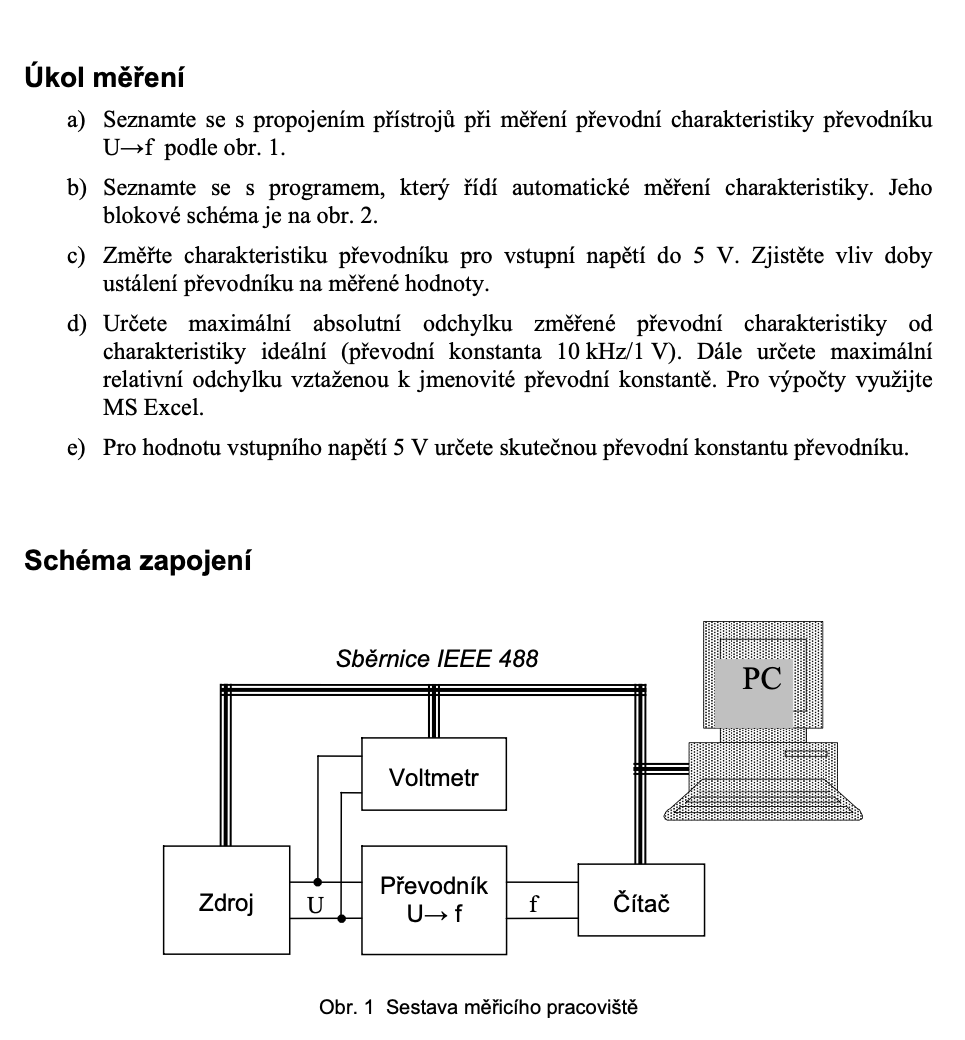
\includegraphics[width=\textwidth]{main.png}
\newpage


\section{Teoretický úvod}
\label{chap:teoreticky_uvod}

V této úloze jsou měřicí přístroje zapojené paralelně do sběrnice IEEE~488. Každý z přístrojů má přiřazenou pětibitovou adresu, pomocí které komunikujeme s danou jednotkou. Nastavování probíhá přes PC. Posloupnost úkonů je následující: Vynulování přístrojů $\rightarrow$ postupné nastavení napětí 0 -- 5~V $\rightarrow$ na programovatelném zdroji $\rightarrow$ odečítání napětí na vstupu $U-f$ převodníku. Data následně zpracujeme v programu MS~Excel.

\section{Naměřené hodnoty}
\label{chap:namerene_hodnoty}
% Please add the following required packages to your document preamble:
% \usepackage[table,xcdraw]{xcolor}
% If you use beamer only pass "xcolor=table" option, i.e. \documentclass[xcolor=table]{beamer}
\begin{table}[h!]
  \begin{tabular}{|l|l|l|l|l|}
  \hline
  Nastavené napětí & Naměřené napětí & Naměřený kmitočet & Odchylka absolutní & Odchylka relativní \\ \hline
  00,5000          & 00,5001         & 4957,0000         & 00,0001            & 00,0002            \\ \hline
  01,0000          & 01,0000         & 9903,0000         & 00,0000            & 00,0000            \\ \hline
  01,5000          & 01,4999         & 14850,0000        & 00,0001            & 00,0001            \\ \hline
  02,0000          & 01,9997         & 19800,0000        & 00,0003            & 00,0002            \\ \hline
  02,5000          & 02,4991         & 24730,0000        & 00,0009            & 00,0004            \\ \hline
  03,0000          & 02,9991         & 29670,0000        & 00,0009            & 00,0003            \\ \hline
  03,5000          & 03,4985         & 34620,0000        & 00,0015            & 00,0004            \\ \hline
  04,0000          & 03,9983         & 39560,0000        & 00,0017            & 00,0004            \\ \hline
  04,5000          & 04,4980         & 44500,0000        & 00,0020            & 00,0004            \\ \hline
  05,0000          & 04,9979         & 49440,0000        & 00,0021            & 00,0004            \\ \hline
  05,5000          & 05,4975         & 54380,0000        & 00,0025            & 00,0005            \\ \hline
  06,0000          & 05,9973         & 59320,0000        & 00,0027            & 00,0005            \\ \hline
  06,5000          & 06,4969         & 64280,0000        & 00,0031            & 00,0005            \\ \hline
  07,0000          & 06,9967         & 69230,0000        & 00,0033            & 00,0005            \\ \hline
  07,5000          & 07,4963         & 74160,0000        & 00,0037            & 00,0005            \\ \hline
  08,0000          & 07,9956         & 79100,0000        & 00,0044            & 00,0005            \\ \hline
  \end{tabular}
  \caption{Tabulka naměřených a vypočtených hodnot hodnot}
  \label{namhod}
  \end{table}

\section{Zpracování naměřených hodnot}
\label{chap:zpracovani_hodnot}
Grafy jsou zobrazené níže.

\begin{figure}
  \centering
  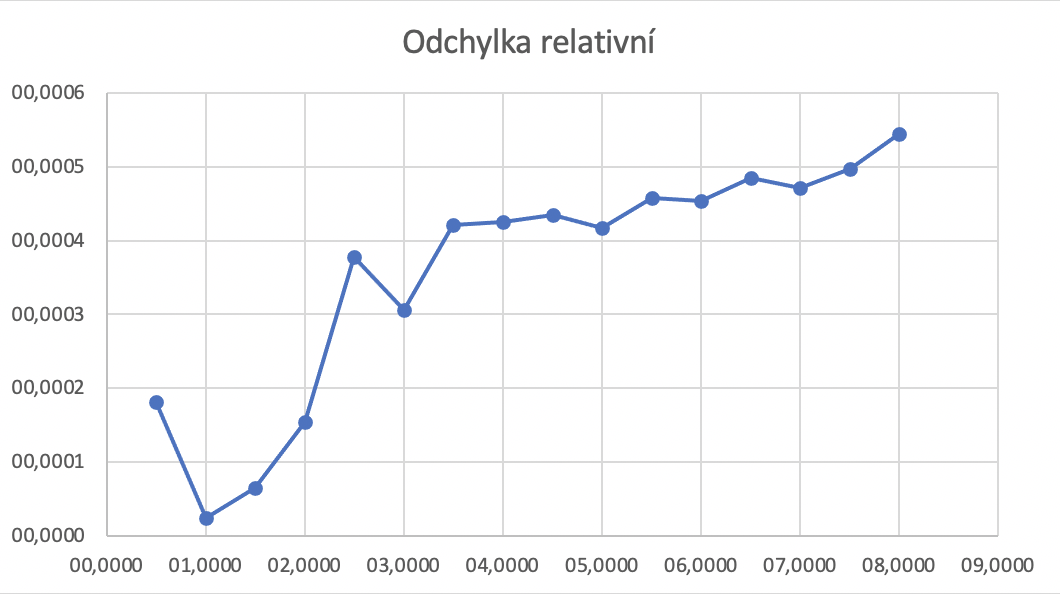
\includegraphics[width=\textwidth]{graf1.png}
  \caption{Závislost měřené odchylky na vstupním napětí}
\end{figure}

\begin{figure}
  \centering
  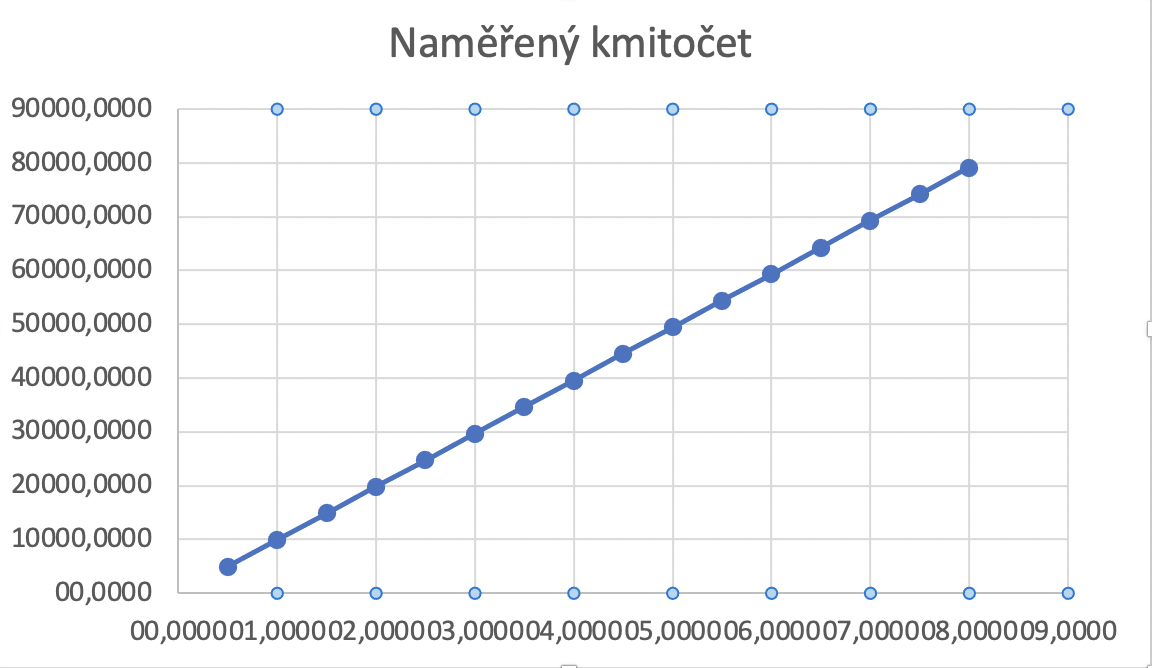
\includegraphics[width=\textwidth]{graf2.png}
  \caption{Závislost frekvence na měřeném napětí}
\end{figure}


\section{Závěrečné vyhodnocení}
\label{chap:zaver}
Z naměřených hodnot je zřejmé, že maximální absolutní odchylka charakteristiky je 56,16~Hz. Maximální relativní odchylka vztažená k převodní konstantě 10~kHz/1~V je 0,05~\%. Skutečná převodní konstanta je je 9896~Hz/V


%--- LITERATURA a~ZDROJE (povinne) ---
\clearpage
\renewcommand{\refname}{Seznam použité literatury a~zdrojů informací} 
%\section*{Seznam použité literatury a~zdrojů informací}
\phantomsection %pridej odkaz do PDF zalozek
\addcontentsline{toc}{section}{Seznam použité literatury a~zdrojů informací}

\begin{thebibliography}{99}

%----------------------------------------------------
\subsection*{Seznam použitých internetových zdrojů}
    \bibitem{navod} Návod k~laboratorní úloze
    
\end{thebibliography}

\end{document}